\documentclass[reqno]{amsart}
\usepackage{amscd, amssymb, amsmath, amsthm}
\usepackage{graphicx}
\usepackage[colorlinks=true,linkcolor=blue]{hyperref}
\usepackage[utf8]{inputenc}
\usepackage[T1]{fontenc}
\usepackage{textcomp}
\usepackage{babel}
%% for identity function 1:
\usepackage{bbm}
%%For category theory diagrams:
\usepackage{tikz-cd}

%\usepackage[backend=biber]{biblatex}
%\addbibresource{.bib}


\setlength\parindent{0pt}

\pdfsuppresswarningpagegroup=1

\newtheorem{theorem}{Theorem}[section]
\newtheorem{lemma}[theorem]{Lemma}
\newtheorem{proposition}[theorem]{Proposition}
\newtheorem{corollary}[theorem]{Corollary}
\newtheorem{conjecture}[theorem]{Conjecture}

\theoremstyle{definition}
\newtheorem{definition}[theorem]{Definition}
\newtheorem{example}[theorem]{Example}
\newtheorem{exercise}[theorem]{Exercise}
\newtheorem{problem}[theorem]{Problem}
\newtheorem{question}[theorem]{Question}

\theoremstyle{remark}
\newtheorem*{remark}{Remark}
\newtheorem*{note}{Note}
\newtheorem*{solution}{Solution}



%Inequalities
\newcommand{\cycsum}{\sum_{\mathrm{cyc}}}
\newcommand{\symsum}{\sum_{\mathrm{sym}}}
\newcommand{\cycprod}{\prod_{\mathrm{cyc}}}
\newcommand{\symprod}{\prod_{\mathrm{sym}}}

%Linear Algebra

\DeclareMathOperator{\Span}{span}
\DeclareMathOperator{\im}{im}
\DeclareMathOperator{\diag}{diag}
\DeclareMathOperator{\Ker}{Ker}
\DeclareMathOperator{\ob}{ob}
\DeclareMathOperator{\Hom}{Hom}
\DeclareMathOperator{\Mor}{Mor}
\DeclareMathOperator{\sk}{sk}
\DeclareMathOperator{\Vect}{Vect}
\DeclareMathOperator{\Set}{Set}
\DeclareMathOperator{\Group}{Group}
\DeclareMathOperator{\Ring}{Ring}
\DeclareMathOperator{\Ab}{Ab}
\DeclareMathOperator{\Top}{Top}
\DeclareMathOperator{\hTop}{hTop}
\DeclareMathOperator{\Htpy}{Htpy}
\DeclareMathOperator{\Cat}{Cat}
\DeclareMathOperator{\CAT}{CAT}
\DeclareMathOperator{\Cone}{Cone}
\DeclareMathOperator{\dom}{dom}
\DeclareMathOperator{\cod}{cod}
\DeclareMathOperator{\Aut}{Aut}
\DeclareMathOperator{\Mat}{Mat}
\DeclareMathOperator{\Fin}{Fin}
\DeclareMathOperator{\rel}{rel}
\DeclareMathOperator{\Int}{Int}
\DeclareMathOperator{\sgn}{sgn}
\DeclareMathOperator{\Homeo}{Homeo}
\DeclareMathOperator{\SHomeo}{SHomeo}
\DeclareMathOperator{\PSL}{PSL}
\DeclareMathOperator{\Bil}{Bil}
\DeclareMathOperator{\Sym}{Sym}
\DeclareMathOperator{\Skew}{Skew}
\DeclareMathOperator{\Alt}{Alt}
\DeclareMathOperator{\Quad}{Quad}
\DeclareMathOperator{\Sin}{Sin}
\DeclareMathOperator{\Supp}{Supp}
\DeclareMathOperator{\Char}{char}
\DeclareMathOperator{\Teich}{Teich}
\DeclareMathOperator{\GL}{GL}
\DeclareMathOperator{\tr}{tr}
\DeclareMathOperator{\codim}{codim}
\DeclareMathOperator{\coker}{coker}
\DeclareMathOperator{\corank}{corank}
\DeclareMathOperator{\rank}{rank}
\DeclareMathOperator{\Diff}{Diff}
\DeclareMathOperator{\Bun}{Bun}
\DeclareMathOperator{\Sm}{Sm}
\DeclareMathOperator{\Fr}{Fr}
\DeclareMathOperator{\Cob}{Cob}
\DeclareMathOperator{\Ext}{Ext}
\DeclareMathOperator{\Tor}{Tor}
\DeclareMathOperator{\Conf}{Conf}
\DeclareMathOperator{\UConf}{UConf}


%Row operations
\newcommand{\elem}[1]{% elementary operations
\xrightarrow{\substack{#1}}%
}

\newcommand{\lelem}[1]{% elementary operations (left alignment)
\xrightarrow{\begin{subarray}{l}#1\end{subarray}}%
}

%SS
\DeclareMathOperator{\supp}{supp}
\DeclareMathOperator{\Var}{Var}

%NT
\DeclareMathOperator{\ord}{ord}

%Alg
\DeclareMathOperator{\Rad}{Rad}
\DeclareMathOperator{\Jac}{Jac}

%Misc
\newcommand{\SL}{{\mathrm{SL}}}
\newcommand{\mobgp}{{\mathrm{PSL}_2(\mathbb{C})}}
\newcommand{\id}{{\mathrm{id}}}
\newcommand{\MCG}{{\mathrm{MCG}}}
\newcommand{\PMCG}{{\mathrm{PMCG}}}
\newcommand{\SMCG}{{\mathrm{SMCG}}}
\newcommand{\ud}{{\mathrm{d}}}
\newcommand{\Vol}{{\mathrm{Vol}}}
\newcommand{\Area}{{\mathrm{Area}}}
\newcommand{\diam}{{\mathrm{diam}}}
\newcommand{\End}{{\mathrm{End}}}


\newcommand{\reg}{{\mathtt{reg}}}
\newcommand{\geo}{{\mathtt{geo}}}

\newcommand{\tori}{{\mathcal{T}}}
\newcommand{\cpn}{{\mathtt{c}}}
\newcommand{\pat}{{\mathtt{p}}}

\let\Cap\undefined
\newcommand{\Cap}{{\mathcal{C}}ap}
\newcommand{\Push}{{\mathcal{P}}ush}
\newcommand{\Forget}{{\mathcal{F}}orget}




\begin{document}

\subsubsection{Exercises}

\begin{exercise}[]
    Let $p \colon E \to B$ be a Serre (resp. Hurewicz) fibration.
    Given any map of spaces $f \colon B' \to B$, show that
    the projection $f^{*}E \to B'$ is a Serre (resp. Hurewicz)
    fibration, where
     \[
     f^{*}(E) = B' \times_B E
     = \left\{ \left( b', e \right)  \mid 
     f(b') = p(e) \right\} 
     \] 
     is the pullback along $f$.
\end{exercise}

\begin{proof}
    Consider the solid part of the diagram
    \begin{equation*}
    \begin{tikzcd}
        X \times \left\{ 0 \right\} \ar[d] \ar[r] 
        \ar[rr, bend left] & f^{*}E \ar[d] \ar[r] & E 
        \ar[d, "p"]\\
        X \times I \ar[r] \ar[rr, bend right]
        \ar[rru, dashed] \ar[ru, dashed]&
        B' \ar[r] & B
    \end{tikzcd}
    \end{equation*}
    In the case where $p$ is a Hurewicz fibration,
    $X$ can be any space, while when $p$ is a Serre
    fibration, it represents any disk $D^{n}$.\\
    We then obtain the first dashed
    arrow $X \times I \to E$ because
    $E \stackrel{p}{\to} B$ is a Hurewicz/Serre fibration.
    But then we have maps
    $X \times I \to B'$ and
    $X \times I \to E$, so by the universal property
    of the pullback, this induces a unique map
    $X \times I \to f^{*} E$ in $\Top$.
\end{proof}

\begin{exercise}[]
    Let $G$ be a topological group and $H$ a subgroup,
    and let $G / H$ have the quotient topology from
    the projection $p \colon G \to G / H$ (here
    $G / H$ is the space of cosets, not the space obtained
    by collapsing $H$ to a point).
    Assume that there exists a nonempty open set
    $U \subset G / H$ such that 
    $p \colon p^{-1}(U) \to U$ admits
    a section $s \colon U \to p^{-1}(U)$. Prove that
    $G \to G / H$ is a fiber bundle. Deduce that
    it is a fibration.
\end{exercise}

\begin{proof}
    By assumption, $p \circ s = \id_U$. 
    Now, picking some $x_0 \in p^{-1}(U)$, the set
    $V:= x_0^{-1} \cdot p^{-1}(U)$ is a neighborhood
    of the identity $e \in G$.
    Let $y \in G / H$, and pick a
    $y_0 \in p^{-1}(y)$. Then
    $y_0 \cdot V$ is a neighborhood of $y_0$, hence
    $p(y_0 \cdot V)$ is a neighborhood of $y$ (it is open
    since $V$ was saturated with respect to $p$ by construciton
    and multiplication by $y_0$ is a homeomorphism of $G$, so
    saturated sets remain saturated).
    Defining
    $s' \colon p(y_0\cdot V) \to 
    y_0 \cdot V $ by
    $s'(\overline{x}) = s \circ p \left( y_0^{-1} \cdot 
    p^{-1}(\overline{x}) \right)  $.
    If $\overline{x} = \overline{z}$, then
    $z^{-1} \cdot x \in H$, so
    $\left( y_0^{-1} \cdot z \right)^{-1} \cdot 
    \left( y_0^{-1} \cdot x \right) \in H$, hence
    $s'\left( \overline{x} \right) 
    = s'\left( \overline{z} \right)$.
    We claim that $s'$ is then also a section
    of $p |_{y_0 V} \colon y_0\cdot 
    V \to p\left( y_0 \cdot V \right) $.
    To see this, we have
    \[
    p \circ s' = 
    p \circ s \circ p \circ \left( y_0^{-1} \cdot - \right) 
    \circ p^{-1}
    = p \circ \left( y_0^{-1} \cdot - \right) \circ
    p^{-1}
    \] 
    Now if $\overline{x} = \overline{z}$ then
    again  $z^{-1}\cdot  x \in H$, so
    $\left( y_0^{-1} \cdot z \right)^{-1} \cdot 
    \left( y_0^{-1} \cdot x \right) \in H$, from which
    the claim follows.\\

    We claim that
    $p^{-1}(U)$ admits a trivialization
    $H \times U \cong p^{-1}(U)$ via the map
    $k \colon 
    \left( h,u \right) \mapsto h \cdot s(u)$. Firstly, this
    is in $p^{-1}(U)$ since
    $p\left( h\cdot s(u) \right) = 
    p\left( s (u) \right) = u \in U$. It is also continuous
    and injective
    as the composition
    $H \times U \stackrel{\id \times s}{\to} 
    H \times p^{-1}(U) \stackrel{\text{prod}}{\to} 
    p^{-1}(U)$.

    Furthermore, if
    $h\cdot v = h' \cdot v$ for some
    $v \in p^{-1}(U)$, then
    $h = h \cdot v \cdot v^{-1} = 
    h' \cdot v \cdot v^{-1} = h'$, so
    the action of $H$ on $U$ is free.

    Suppose
    $h \cdot s(U) \cap
    h' \cdot s(U) \neq \varnothing$, so for
    some $u,u' \in U$,
    $h\cdot s(u) = h' \cdot s(u')$. But then
    $u = p \left( h \cdot s(u) \right) =
    p\left( h' \cdot s(u') \right) 
    = u'$, and so
    $h = h \cdot s(u) \cdot s(u)^{-1} =
    h' \cdot s(u) \cdot s(u)^{-1} = h'$.
    Hence
    $p^{-1}(U) = 
    \sqcup_{h \in H} h\cdot s(U)$. Now define
    $r \colon p^{-1}(U) \to H \times U$ by
    $r (u) = \left( \sum_{h \in H}
    h \cdot \delta_{u \in h\cdot s(U)}, p(u) \right) $.
    Then
    \[
    r \circ k(h,u) =
    r \left( h \cdot s(u) \right) 
    = \left( h, u \right) 
    \] 
    and
    \[
    k \circ r \left( x \right) 
    = k \left( h,u \right) 
    = x
    \] 
    since $(h,u)$ are by definition such that
    $p(x) = u$ and
    $x \in h \cdot s(U)$, so we
    must have $x = h\cdot s (u)$. Thus
    $k (h,u) = h \cdot s(u) = x$. 
    So $r$ is an inverse function to $k$. It remains to show
    that it is continuous. The
    coordinate $p(u)$ is continuous, so
    we must show that
    $r_1 \colon u \mapsto \sum_{h \in H} h \cdot \delta_{u \in 
    h \cdot s(U)}$ is continuous. For this,
    note that for an open set
    $W \subset H$, $r_1^{-1} (W)
    = \bigcup_{h \in W} h\cdot s(U)$. Now,
    since $p \left( h \cdot s(u) \right) =
    p(s(u)) = u $, so
    $r_1^{-1}(W) \subset p^{-1}(U)$, and
    conversely, for any
    $x \in p^{-1}(U)$, there is an $h\in H$ such that
    $x \in h \cdot s(U)$, so
    $p^{-1}(U) \subset \bigcup_{h \in W}  h\cdot s(U)$.
    Hence $r_1^{-1}(W) = p^{-1}(U)$ which is open.
    
    This completes the proof that
    $G \to G /H$ is a fiber bundle.

    Since any fiber bundle is a fibration, the last part follows
    directly.


\end{proof}


\begin{exercise}[]
    Recall that $S^3 \subset \mathbb{R}^{4} \cong
    \mathbb{H} $ is a topological group, with
    $S^{1} \subset \mathbb{C} \subset \mathbb{H}$ as a topological
    subgroup.
    Recall that
    \[
    \mathbb{H} = \left\{ 
    a + bi + cj + dk  \mid a,b,c,d \in \mathbb{R} \right\} .
    \] 
    so $S^{3} \subset \mathbb{H}$ here
    is considered as the group whose
    elements are elements in $\mathbb{H}$ with
    norm $1$, and
    $S^{1} \subset S^3$ as the subgroup
    \[
    \left\{ a+bi  \mid  a^2+ b^2 = 1 \right\} .
    \] 
    \begin{enumerate}
        \item Prove (using the previous exercise)
            that $S^3 \to S^3 / S^{1}$ is a fiber bundle
            with fiber $S^{1}$, and therefore a fiber bundle.
        \item Prove that $S^3 / S^{1} \cong S^2$. The
            fiber sequence $S^{1} \to S^3 \to S^2$ is
            called the \textit{Hopf} fibration.
        \item Use the LES associated to this fibration
            to compute $\pi_3 (S^2)$.
        \item Show that $S^3 \times K(\mathbb{Z},2)$ and
            $S^2$ have isomorphic homotopy groups. Are
            they homotopy equivalent?
    \end{enumerate}
\end{exercise}



\begin{proof}
    (1) Let
    $S_+^{3}$ denote the open upper hemisphere.
    Then if $p \colon S^3 \to S^3 / S^{1}$ is the quotient map,
    $S^3 / S^{1}$ looks 
\end{proof}




\newpage


\maketitle

\subsubsection{Problems}


    \begin{problem}[]
        Suppose $p \colon E \to B$ is a Serre
        fibration and $f \colon X \to B$ is
        $n$-connected. Prove that the projection
        $E \times_B X \to E$ is also $n$-connected.
    \end{problem}

    \begin{proof}
        We are given the following commutative diagram
        \begin{equation*}
        \begin{tikzcd}
            E \times_B X \ar[r] \ar[d] & E \ar[d, "p"] \\
            X \ar[r, "f"'] & B
        \end{tikzcd}
        \end{equation*}
        Firstly, by Exercise 1 on Problem set 4, 
        the map
        $E \times_B X \to X$ is also a
        Serre fibration.\\
        Secondly, by assumption in the conventions section
        for problem set 4, all spaces
        are assumed to be locally path-connected and connected,
        hence all spaces are path-connected. In 
        particular, both $X$ and $B$ are assumed to be
        path-connected, so
        by Theorem 4.41 in Hatcher, we have a LES
        \[
        \ldots \to 
        \pi_k (F',y_0) \to 
        \pi_k(E \times_B X, y_0) 
        \stackrel{(\pi_X)_*}{\to} \pi_k (X,x_0)
        \to \pi_{k-1}(F',y_0) \to \ldots \to 
        \pi_0 \left( E \times_B X, y_0 \right)  \to 0
        \] 
        where
        $F' = \left( \pi_X \right)^{-1}(x_0)$ for
        some $x_0 \in X$
        and $y_0 \in F'$.
        Now,
        \[
        F' = 
        \left( \pi_X \right)^{-1}(x_0)
        = \left\{ \left( e,x_0 \right)  \mid 
        f(x_0) = p(e)  \right\} 
        \xrightarrow[\cong]{\pi_E}  p^{-1}\left( f(x_0) \right) =: 
        F
        \] 
        where we choose $F$ to be
        the fiber of $p \colon E \to B$ (when repeating
        Theorem 4.41 for this fibration), and
        we choose 
        $e_0 \in F$ to be
        $\pi_E (y_0)$.
        With these choices of fibers and basepoints, we
        obtain that the map
        $\pi_E|_{F'} \colon F' \to F$ is a homeomorphism
        (it has the inverse
        $e \mapsto (e, x_0)$ )
        by construction, so the following
        diagram commutes:

        \begin{equation*}\tag{$\Omega$}\label{Omega}
        \begin{tikzcd}
            (F',y_0) \ar[r, "\cong"] \ar[d, hookrightarrow]
            & (F,e_0) \ar[d, hookrightarrow] \\
            (E \times_B X, y_0) \ar[d, "\pi_X"] \ar[r, "\pi_E"]
            & (E,e_0) \ar[d, "p"] \\
            (X,x_0) \ar[r, "f"] & (B,f(x_0))
        \end{tikzcd}
        \end{equation*}
        


        With these choices of basepoints,
        Theorem 4.41 gives the following long exact sequences
        (the solid part of the diagram)
        \begin{equation*}\tag{$\Gamma$}\label{Gamma}
        \begin{tikzcd}
            \pi_{k+2}(X,x_0) \ar[d, dashed]
            \ar[r] & \pi_{k+1}(F',y_0) \ar[r] \ar[d, dashed] & 
            \pi_{k+1}(E \times_B X, y_0) \ar[r, "(\pi_X)_*"] 
            \ar[d, dashed] &
            \pi_{k+1}(X,x_0) \ar[r] \ar[d, dashed] & 
            \pi_k (F',y_0) \ar[d, dashed] \\
            \pi_{k+2}(B, f(x_0) \ar[r] & \pi_{k+1}(F, e_0) \ar[r] & 
            \pi_{k+1}(E,e_0) \ar[r, "p_*"] &
            \pi_{k+1}(B,f(x_0)) \ar[r] &
            \pi_{k}(F,e_0)
        \end{tikzcd}
        \end{equation*}

        Now, applying $\pi_{k+1}$ to 
        \eqref{Omega}, i.e., using functoriality of
        $\pi_{k+1}$ on pointed topological spaces,
        we find that for
        $k+1 \ge 1$, we have

        
        \begin{equation*}\tag{$\zeta$}\label{zeta}
        \begin{tikzcd}
            \pi_{k+1}(F', y_0) \ar[r, "\cong"] \ar[d]
            & \pi_{k+1}(F,e_0) \ar[d] \\
            \pi_{k+1}(E \times_B X, y_0)
            \ar[d, "(\pi_X)_*"] \ar[r, "(\pi_E)_*"]
            & \pi_{k+1}(E,e_0) \ar[d, "p_*"] \\
            \pi_{k+1}(X,x_0) \ar[r, "f_*", "\cong"']
            & \pi_{k+1}(B,f(x_0))
        \end{tikzcd}
        \end{equation*}
        commutes (since functoriality of $\pi_{k+1}$ implies
        that compositions are preserved) - where
        also $f_*$ is an isomorphism for
        $k < n-1$ and surjective for
        $k = n-1$.\\
        We now claim that
        \begin{equation*}
        \begin{tikzcd}
            \pi_{k+1}(X,x_0) \ar[r] \ar[d, "f_*"] &
            \pi_k (F',y_0) \ar[d, "(\pi_E|_{F'})_*",
            "\cong"']\\
            \pi_{k+1}(B,f(x_0)) \ar[r] & 
            \pi_{k}(F,e_0)
        \end{tikzcd}
        \end{equation*}
        commutes.
        Consider the following diagram:

        \begin{equation*}
        \begin{tikzcd}
            \pi_{k+1}(E \times_B X, F') \ar[r, "(\pi_X)_*",
            "\cong"']
            \ar[rr, bend left, "\partial"] 
            \ar[d, "(\pi_E)_*"]& 
            \pi_{k+1}(X,x_0) \ar[r] \ar[d, "f_*"]&
            \pi_k(F',y_0) \ar[d, "(\pi_E|_{F'})_*"] \\
            \pi_{k+1}(E, F) \ar[r, "p_*", "\cong"']
            \ar[rr, bend right,
            "\partial"] &
            \pi_{k+1}(B, f(x_0)) \ar[r] &
            \pi_k (F,e_0)
        \end{tikzcd}
        \end{equation*}
        The outer triangle commutes by construction:
        since for $g \colon
        \left( D^{n+1}, S^{n}, s_0 \right) 
        \to \left( E \times_B X, F', y_0 \right) $,
        we get
        \[
          \partial \circ
          \left( \pi_E \right)_*
          \left( \left[ g \right]  \right) 
          =\partial \left[ \pi_E \circ g \right] 
        = \left[ \left( \pi_E \circ g \right)|_{S^{n}} \right] 
        = \left[ \pi_E|_{F'} \circ g|_{S^{n}} \right]
        = \left( \pi_E|_{F'} \right)_*
        \left( \left[ g|_{S^{n}} \right]  \right) 
        = \left( \pi_E|_{F'} \right)_*
    \circ \partial \left( \left[ g \right]  \right).
\]
Also, the left hand square commutes for $k+1\ge 1$, since
this is what we obtained from \eqref{zeta}.
From this, we can conclude that the right hand square
also commutes for $k+1\ge 1$, i.e., for $k\ge 0$.
Explicitly, if we let
$k$ be the map
$\pi_{k+1}(X,x_0) \to \pi_{k}(F',y_0)$ and
$l$ the map
$\pi_{k+1}(B,f(x_0)) \to \pi_k (F,e_0)$, then we
get
\begin{align*}
    (\pi_E|_{F'})_* \circ j
    &= (\pi_E|_{F'})_* \circ \partial \circ
    \left( \pi_X \right)_*^{-1}\\
    &= \partial \circ (\pi_E)_* \circ (\pi_X)_*^{-1}\\
    &= \partial \circ p_*^{-1} \circ f_*\\
    &= l \circ f_*
\end{align*}
giving commutativity.\\
        

        Therefore, we can fill in the dashed arrows
        in diagram \eqref{Gamma}, giving that the
        following diagram commutes
        for $0\le k < n-1$.

        \begin{equation*}
            \begin{tikzcd}
                \pi_{k+2}(X,x_0) \ar[d, "f_*", twoheadrightarrow]
                \ar[r] & \pi_{k+1}(F',y_0) \ar[r] \ar[d,
            "\cong", "(\pi_E|_{F'})_*"'] & 
            \pi_{k+1}(E \times_B X, y_0) \ar[r, "(\pi_X)_*"] 
            \ar[d, "(\pi_E)_*"] &
            \pi_{k+1}(X,x_0) \ar[r] \ar[d, "f_*"',
            "\cong"] & 
            \pi_k (F',y_0) \ar[d, "\cong"] \\
            \pi_{k+2} (B, f(x_0)) \ar[r] & \pi_{k+1}(F, e_0) \ar[r] & 
            \pi_{k+1}(E,e_0) \ar[r, "p_*"] &
            \pi_{k+1}(B,f(x_0)) \ar[r] &
            \pi_{k}(F,e_0)
        \end{tikzcd}
        \end{equation*}

        By the $5$-lemma, we
        obtain that
        $\left( \pi_E \right)_* \colon
        \pi_{k+1}(E \times_B X, y_0)
        \to \pi_{k+1}(E,e_0)$ is an isomorphism
        for $1 \le k+1 \le n-1$.
        Note that this also works
        for $1 = k+1$ despite $\pi_0$ not being
        a group (one can simply trace through the
        arguments in the proof of the $5$-lemma and
        see that it still works with exactly
        the same arguments).



        It remains to show that it
        is an isomorphism on $\pi_0$ and
        surjective on $\pi_n$.
        Surjectivity on $\pi_n$ 
        immediately follows by applying the
        $4$-lemma to the following diagram:
        
        \begin{equation*}
            \begin{tikzcd}
               \pi_{n}(F',y_0) \ar[r] \ar[d,
            "\cong", "(\pi_E|_{F'})_*"'] & 
            \pi_{n}(E \times_B X, y_0) \ar[r, "(\pi_X)_*"] 
            \ar[d, "(\pi_E)_*"] &
            \pi_{n}(X,x_0) \ar[r] \ar[d, "f_*"',
            "\cong"] & 
            \pi_{n-1} (F',y_0) \ar[d, "\cong"] \\
            \pi_{n}(F, e_0) \ar[r] & 
            \pi_{n}(E,e_0) \ar[r, "p_*"] &
            \pi_{n}(B,f(x_0)) \ar[r] &
            \pi_{n-1}(F,e_0)
        \end{tikzcd}
        \end{equation*}

        For the isomorphism on
        $\pi_0$, note that we have
        assumed that $E$ is path-connected, so it
        suffices to show that
        the induced map
        $(\pi_E)_* \colon
        \pi_0 \left( E \times_B X, y_0 \right) \to 
        \pi_0 (E,e_0) = 0$ is injective.
        Since the diagram (footnote: \footnote{In this diagram,
        when we are talking about exactness of the rows,
        while $\pi_0$ of the spaces are not groups, we
    can still define exactness and exact sequences of
pointed sets as one might expect: 
$\left( X,x \right) \stackrel{f}{\to} 
\left( Y,y \right) \stackrel{g}{\to} (Z,z)$ is
exact if the composite $gf$ is constant at
$z$ and $g(a) = z$ implies that
there a $b$ with $a = f(b)$})

        \begin{equation*}
        \begin{tikzcd}
            \pi_1(X,x_0) \ar[d, "f_*", "\cong"'] \ar[r] &
            \pi_0(F',y_0) \ar[r] \ar[d, "\cong"'] 
            & \pi_0 (E \times_B
            X,y_0) \ar[d, "(\pi_E)_*"] \ar[r] &
            0\\
            \pi_1 (B,f(x_0)) \ar[r] & \pi_0(F,e_0) \ar[r] &
            \underbrace{\pi_0 (E,e_0)}_{0} \ar[r] & 0
        \end{tikzcd}
        \end{equation*}
        commutes with exact rows, we obtain by the
        $4$-lemma that 
        $(\pi_E)_* \colon
        \pi_0 \left( E \times_B X,y_0 \right) \to 
        \pi_0(E,e_0) =0$ is injective, so in particular
        $\pi_0 \left( E\times_B X,y_0 \right) = 0$.
        Note that the part of the $4$-lemma which we
        used (the one concluding monomorphism) does
        not require the objects to be groups or, for that
        matter, the diagram to be in an abelian category - 
        we just need the kernel to be concrete. 
        (See footnote \footnote{For concreteness,
        what I am saying is that all the steps in the
    proof of the $4$-lemma as laid out for example on
Wikipedia (\url{https://en.wikipedia.org/wiki/Five_lemma}) all
still hold in our situation ad verbum, hence
I do not wish to repeat all the arguments since it's just a
lengthy diagram chase. One thing to note, however, is
that when we talk about $0$ in $\pi_0$ in the arguments,
this means to be in the same path-component as
the basepoint. With this terminology, all things go through.}).
        Thus $(\pi_E)_*$ is an isomorphism on
        $\pi_0$ also.\\
        \linebreak
        This completes the proof.
    \end{proof}

    \begin{problem}[]
        The (ordered) configuration space on
        $n$-points of a space
        $X$ is the subspace
        \[
        \Conf_n (X) = 
        \left\{ \left( x_1, \ldots, x_n \right) \in X^{n}
         \mid \forall i\neq j \colon
     x_i \neq x_j \right\} \subset X^{n}
        \] 
        of those $n$-tuples of points that are
        pairwise distinct. In this problem, we consider
        the special case $X = \mathbb{R}^2$. You may assume
        that the map
        \begin{align*}
            \Conf_n (\mathbb{R}^2) 
            &\to \Conf_{n-1}(\mathbb{R}^2)\\
            \left( x_1,\ldots, x_n \right) 
            &\mapsto \left( x_1, \ldots, x_{n-1} \right) 
        \end{align*}
        is a fiber bundle. We define
        the base-point of $\Conf_n (\mathbb{R}^2)$ to
        be $x = \left( (1,0), (2,0) ,\ldots,
        (n,0)\right) $.\\

        
        \begin{enumerate}
            \item Show that $\Conf_n (X)$ is an Eilenberg-MacLane
        space of type $(G,1)$ with $G = \pi_1 \Conf_n (\mathbb{R}^2)$.\\
        \linebreak
        For $1 \le i < j \le n$, define elements
        $\gamma_{i,j} \in \pi_1 \Conf_n (X)$ as follows:
        \[
        \gamma_{i,j}(t) = \left( (1,0),
        \ldots, (i-1,0), \rho(t), (i+1,0), \ldots,
    (n,0) \right) 
        \] 
        where $\rho \colon \left[ 0,1 \right] \to \mathbb{R}^2$ 
        is a loop that starts and ends at $(i,0)$ and loops
        around $(j,0)$ and avoids the other points.\\
    \item Show that the  $\gamma_{i,j}$ generate
        $\pi_1 \Conf_n (\mathbb{R}^2)$.\\
        \linebreak
        The unordered configuration space is defined as
        the set of subsets of $\mathbb{R}^2$ of cardinality
        $n$ :
        \[
        \UConf_n (\mathbb{R}^2)
        = \left\{ A \subset \mathbb{R}^2  \mid 
        \left| A \right| = n\right\} .
        \] 
        This is topologised with the quotient topology
        coming from the map $\Conf_n (\mathbb{R}^2) \to 
        \UConf_n (\mathbb{R}^{n})$ sending
        $\left( x_1,\ldots, x_n \right) $ to
        $\left\{ x_1,\ldots, x_n \right\} $.\\
        \linebreak
    \item Show that $\UConf_n (X)$ is an Eilenberg-MacLane space
        of type $(G,1)$ with $G = \pi_1 \UConf_n (\mathbb{R}^2)$.
        \end{enumerate}


    \end{problem}


    \begin{proof}
        (1) The fiber above the base point
        $\left( x_1,\ldots,x_{n-1} \right) 
        \in \Conf_{n-1}(\mathbb{R}^2)$ under the map
        is
        $F = \left\{ \left( x_1,\ldots,x_n \right)  \mid 
        \forall i\colon x_n \neq x_i\right\} \cong 
        \mathbb{R}^2 - \left\{ x_1,\ldots,x_{n-1} \right\} $.
        Since every fiber bundle is a Serre fibration, we
        find from the LES associated to the fibration that

        \[
        \pi_k \left( \mathbb{R}^2 - \left\{ x_1,\ldots,
        x_{n-1}\right\}  \right) \to 
        \pi_k \left( \Conf_n (\mathbb{R}^2) \right) 
        \to \pi_k \left( \Conf_{n-1}(\mathbb{R}^2) \right) 
        \to \pi_{k-1}\left( \mathbb{R}^2 - 
        \left\{ x_1,\ldots, x_{n-1} \right\} \right) .
        \] 
        is exact for all
        $k \ge 1$.

        By theorem 4.41, if
        $\Conf_{n-1}(\mathbb{R}^2)$ is path-connected, then
        \[
        \underbrace{\pi_0 \left( \mathbb{R}^2 - \left\{ x_1,\ldots,
        x_0\right\}  \right)}_{0} \to 
        \pi_0 \left( \Conf_n (\mathbb{R}^2) \right) 
        \to 0
        \] 
        is exact, 
        so $ \pi_0 \left( \Conf_n (\mathbb{R}^2) \right) 
        \cong 0$. Now,
        $\Conf_1 (\mathbb{R}^2) = \mathbb{R}^2$ which
        is path-connected, so by induction,
        $\Conf_n (\mathbb{R}^2)$ is path-connected for
        all $n\ge 1$, hence
        $\pi_0 \left( \Conf_n \left( \mathbb{R}^2 \right)  \right) =
        0$.\\


        Now, $\mathbb{R}^2 - \left\{ x_1,\ldots,x_{n-1} \right\} 
        \simeq \bigvee_{n-1}S^{1}$.
        In particular, the universal cover of a graph
        is a tree hence contractible, so since
        $\pi_k \left( \bigvee_{n-1}S^{1} \right) $ 
        coincides with $\pi_k$ of the universal cover
        when $k\ge 2$, we find that
        $\pi_k \left( \mathbb{R}^2 - \left\{ x_1,
        \ldots, x_{n-1}\right\}  \right) \cong 0$ for
        $k\ge 2$.
        Thus
        $\pi_k \left( \Conf_n \left( \mathbb{R}^2 \right) 
        \right) \cong
        \pi_k \left( \Conf_{n-1}(\mathbb{R}^2) \right) $ for
        all $k\ge 2$.
        By repeated application, we thus get
        that
        $\pi_k \left( \Conf_n \left( \mathbb{R}^2 \right) 
        \right) \cong
        \pi_k \left( \Conf_1 \left( \mathbb{R}^2 \right)  \right) 
        \cong \pi_k \left( \mathbb{R}^2 \right) 
        \cong 0$ for $k\ge 2$ since
        $\Conf_1\left( \mathbb{R}^2 \right) = 
        \mathbb{R}^2$.\\

        It remains to show that
        $\pi_1 \Conf_n (\mathbb{R}^2) \neq 0$.
        Noting that
        $\pi_0 \left( \Conf_n (\mathbb{R}^2) \right) \cong 0$ 
        and $\pi_2 \left( \Conf_{n-1}(\mathbb{R}^2) \right) $,
        we obtain from the LES associated
        to the fibration
        $\Conf_n (\mathbb{R}^2) \to \Conf_{n-1}\left( \mathbb{R}^2
        \right) $ the following exact sequence:
        \[
        0 \to \pi_1 \left( \mathbb{R}^2 - 
        \left\{ x_1, \ldots, x_{n-1} \right\} \right) 
        \to \pi_1 \Conf_n \left( \mathbb{R}^2 \right) 
        \to \pi_1 \Conf_{n-1} \left( \mathbb{R}^2 \right) \to 0
        \] 
        Now,
        $\pi_1 \left( \mathbb{R}^2
        - \left\{ x_1,\ldots, x_{n-1} \right\} \right) 
        \cong \pi_1 \left( \bigvee_{n-1} S^{1} \right) 
        \cong F_{n-1} = 
        \left< x_1, \ldots, x_{n-1} \right>$, the
        free group on $n-1$ elements.
        Now, when $n=1$,
        $\Conf_n \left( \mathbb{R}^2 \right) =
        \mathbb{R}^2$, so
        $\pi_1 \Conf_1 \left( \mathbb{R}^2 \right) \cong 0$, and
        hence
        $\pi_1 \Conf_2 \left( \mathbb{R}^2 \right) 
        \cong F_1 \cong \mathbb{Z}$. But free groups are
        projective, so by induction, the exact sequence
        \[
        0 \to F_{n-1} \to \pi_1 \Conf_n \left( \mathbb{R}^2 \right) 
        \to \pi_1 \Conf_{n-1} (\mathbb{R}^2) \to 0
        \tag{$\xi$}\label{xi}
        \] 
        splits, hence each
        $\pi_1 \Conf_n (\mathbb{R}^2)$ is non-trivial as
        it contains an isomorphic copy of a free group.
        This shows that $\Conf_n (\mathbb{R}^2)$ is
        a $K(G,1)$ space for all $n\ge 1$.\\
        We will even show below that the SES 
        in \eqref{xi} splits.\\
        \linebreak
        (2)

        \begin{note}
            Below, we will abuse terminology by identifying
            $F_{n-1}$ with
            $\pi_1 \left( \mathbb{R}^2 - \left\{ x_1,
            \ldots, x_{n-1} \right\}  \right) $ and
            $\iota_n$ having either as a domain.

            Furthermore, these are always pointed maps.
        \end{note}

        To find generators, we first look at the
        actual maps in the LES for the fiber bundle.
        Let $p_n \colon
        \Conf_n (\mathbb{R}^2) \to 
        \Conf_{n-1} \left( \mathbb{R}^2 \right) $ be
        the map that forgets the last coordiante, and
        and let 
        $\iota_n \colon  
        \mathbb{R}^2 - \left\{ x_1,\ldots,x_{n-1}  \right\} 
        \cong F \hookrightarrow 
        \Conf_n \left( \mathbb{R}^2 \right) $ be
        the inclusion of the fiber.\\

        We now show that 
        \eqref{xi} splits. Define a map
        $s \colon
        \Conf_{n-1}\left( \mathbb{R}^2 \right) 
        \to \Conf_n \left( \mathbb{R}^2 \right) $ by
        $s\left( x_1, \ldots, x_{n-1} \right) 
        = \left( x_1,\ldots, x_{n-1},
        x_n'\right) $ where
        $x_n' = (1 + \max_{i\le n-1} \left| x_i \right|, 0) $. This
        map is continuous since the norm is
        continuous, and we also have
        $p \circ s = \id_{\Conf_{n-1}\left( \mathbb{R}^2 \right) }$.
        Since both $p$ and $s$ preserve
        basepoints, we find by taking $\pi_1$ that
        $p_* \circ s_* = 
        \id_{\pi_1 \Conf_{n-1} \left( \mathbb{R}^2 \right) }$.
        That is, $s_*$ is a section, so
        \eqref{xi} splits.\\
         \linebreak
        





         Thus we have
        \[
        F_{n-1} \oplus \pi_1 \Conf_{n-1}(\mathbb{R}^2)
        \cong \pi_1 \Conf_n (\mathbb{R}^2)
        \] 
        under the isomorphism
        $(x,y) \mapsto \left( \iota_n \right)_*(x) +
        s_*(y)$.
        Since $\pi_1 \Conf_2 \left( \mathbb{R}^2 \right) 
        \cong \pi_1 S^{1}$ induced by the deformation retract
        $\mathbb{R}^2 -\left\{ x_1 \right\} 
        \times I \to  \mathbb{R}^2 - \left\{ x_1 \right\} $ sending
        $\left( x,t \right) \mapsto 
        (1-t) (x-x_1) + t \frac{x-x_1}{\|x - x_1\|} + x_1$.
        Under this isomorphism, we see that 
        $\gamma_{1,2}$ which winds
        around the puncture once corresponds to
        a generator for $\pi_1 S^{1}$ - namely a loop that
        goes once around.
        Thus $\gamma_{1,2}$ indeed generates
        $\pi_1 \Conf_2 \left( \mathbb{R}^2 \right) $.\\
        Now, suppose we have
        shown for $n \le N-1$ that
        $\pi_1 \Conf_n \left( \mathbb{R}^2 \right) $ 
        is generated by
        $\left\{ \gamma_{i,j} \right\}_{1 \le i < j \le n}$.
        Then using the isomorphism
        \[
        \pi_1 \left(F \right)  \oplus \pi_1 \Conf_{N-1}\left( \mathbb{R}^2 \right) 
        \stackrel{\left( x,y \right) \mapsto 
        \iota_{N*}(x) +s_* (y)}{\to} \pi_1 \Conf_N 
        \left( \mathbb{R}^2 \right) 
        \] 
        we see that the
        $\gamma_{i,j} \in 
        \pi_1 \Conf_{N-1} \left( \mathbb{R}^2 \right)$ 
        are mapped under the isomorphism to
        $\gamma_{i,j} \in 
        \pi_1 \Conf_{N-1}\left( \mathbb{R}^2 \right) $ 
        (we will furthermore assume that the given
        $\rho $ which loop around $(j,0)$ from $(i,0)$ are
        sufficiently close to he the other points
        $(1,0) ,\ldots, (N,0)$ at all times so that
        $1 + \max_{i \le N-1} \left| x_i \right| $ will
        be equal to $(N,0)$):

        \[
            \gamma_{i,j}(t) =
        \left( (1,0) ,\ldots, (i-1,0) ,
        \rho(t), (i+1,0) , \ldots, \underbrace{(1 + 
    \max_{i\le N-1} \left| x_i \right| ,0)}_{(N,0)} \right)
\]

        So to complete the induction, it suffices to show
        that the remaining loops
        $\gamma_{i,N}$ correspond to generators of
        $F_{n-1}$. The problem is that under the isomorphism
        above, a loop  $\alpha_{i} \in 
        \pi_1 \left( \mathbb{R}^2 - \left\{ x_1, \ldots,
        x_{N-1}\right\}  \right) $, which winds once
        around $x_i$ and then returns to the basepoint, corresponds
        to the loop
        in $\pi_1(F)$ whose $N-1$ first coordinates remain
        fixed at $x_1, \ldots, x_{N-1}$ and where
        the last coordinate traces out a loop
        where it winds around $x_i$ once and then returns back
        to the basepoint $x_N$.
        Hence all of the loops
        in $\pi_1 (F)$ are not of the form
        $\gamma_{i,N}$. 
        However, we claim that the loop is homotopic
        to a $\gamma_{i,N}$.

        To see this, we will regard 
        $\pi_1 \Conf_N \left( \mathbb{R}^2 \right) $ 
        in a different way.
        The group $\pi_1 \Conf_N \left( \mathbb{R}^2 \right) $ 
        is commonly called the pure braid group
        $PB_N$. To visualize a loop
        $\alpha \colon \left( I, \left\{ 0,1 \right\}  \right) 
        \to \pi_1 \left( \Conf_N (\mathbb{R}^2),
         \left( (1,0), \ldots, (N,0) \right)  \right) $ 
         consider 
         $\alpha$ as
         $\alpha(t) = 
         \left( \alpha_1(t), \ldots,
         \alpha_N(t) \right) $ where
         $\alpha_i(t)$ is the $i$ th coordinate
         of $\alpha$.
         This $\alpha_i$ traces out a loop in
         $\mathbb{R}^2$
         in the common sense.
         Define now a new map
         $\beta_i \colon I \to 
         \mathbb{R}^2 \times I$
         by $\beta_i (t) = 
         \left( \alpha_i(t), t \right) $. Then
         $\left( \beta_1, \ldots, \beta_N \right) $ is a braid.
         See Figure \ref{fig:Figures-braid-diagram-jpg}
         for a typical example in
         $\pi_1 \Conf_3 \left( \mathbb{R}^2 \right) $.

         \begin{figure}[htpb]
             \centering
             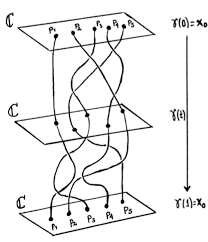
\includegraphics[width=0.5\textwidth]{Figures/braid-diagram.png}
             \caption{Here $\mathbb{C}$ can be replaced
             with $\mathbb{R}^2$.}
             \label{fig:Figures-braid-diagram-jpg}
         \end{figure}

         So how do the loops
         in the image of
         $\left( \iota_N \right)_* $ look like?
         Well, since the first $N-1$ coordinates are
         constant, our $\beta_i$ are of the form
         $\beta_i (t) = 
         \left( (i,0), t \right) $ for $i \le N-1$.
         And since $\alpha_N$ by construction traced
         out a loop that went around
         one of the punctures $(i,0)$ and not the others, 
         $\beta_N$ will be a strand which starts
         at $\left( (N,0),0 \right) $ then which wraps (in a
         continuous level-wise manner) around
         the $i$ th braid once and the connects
         to $\left( (N,0),1 \right) $.
         See Figure \ref{fig:braid2-jpg} 
         \begin{figure}[htpb]
             \centering
             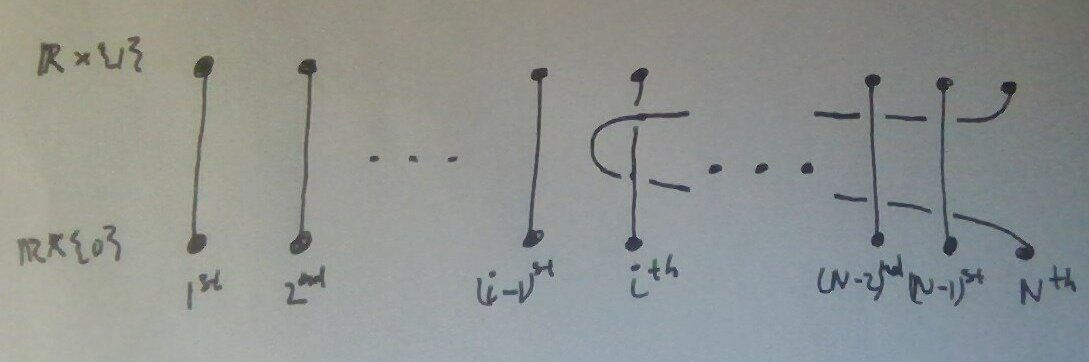
\includegraphics[width=1\textwidth]{Figures/braid2.jpg}
             \caption{}
             \label{fig:braid2-jpg}
         \end{figure}
         Now, what is a homotopy in
         $\pi_1 \Conf_n \left( \mathbb{R}^2 \right) $?
         It will have the form
         $\left( F_1(x,t), \ldots, F_N(x,t) \right) $ where
         $F_i \colon
          I \times I \to \mathbb{R}^2$
          depicts a loop. Furthermore,
          at each time $t_0 \in I$,
          $F_i(x,t_0) \neq F_j(x,t_0)$; i.e.,
          the braids are disjoint/non-intersecting.
          Hence a homotopy in $\pi_1 \Conf_n(\mathbb{R}^2)$ 
          is the same as an isotopy of the braid
          that the loop depicts.

          With this setup in mind, we can now show that
          the loop in Figure \ref{fig:braid2-jpg} is
          homotopic to $\gamma_{i,N}$.
          This, in particular, is equivalent to saying that
          the braid in \ref{fig:braid2-jpg} is isotopic
          to the braid the $\gamma_{i,N}$ corresponds to.
          To see this, consider the isotopy depicted in
          Figure \ref{fig:braid3-jpg}.

          \begin{figure}[htpb]
              \centering
              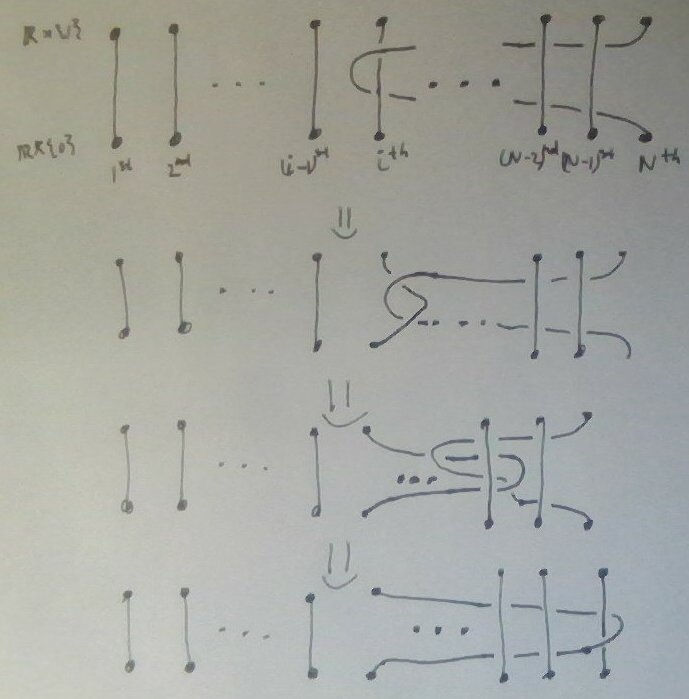
\includegraphics[width=0.8\textwidth]{Figures/braid3.jpg}
              \caption{}
              \label{fig:braid3-jpg}
          \end{figure}
          
          At the bottom, we obtain
          $\gamma_{i,N}$. Thus
           $\im \left( \iota_N \right)_*$ indeed
           corresponds to the remaining
           $\gamma_{i,j}$ 's.\\
           And this completes the inductive argument.\\
           \linebreak
           (3) 
           As we equip $\UConf_n \left( \mathbb{R}^{2} \right) $
           with the quotient topology obtained from
           the map
           $\Conf_n \left( \mathbb{R}^2 \right) \to 
           \UConf_n \left( \mathbb{R}^2 \right) $, this
           map becomes continuous, and as 
           $\Conf_n \left( \mathbb{R}^2 \right) $ was
           path-connected and continuous images of
           path-connected spaces are path-connected, we
           find that
           $\pi_0 \UConf_n \left( \mathbb{R}^2 \right) =0$
           for all $n$. Next,
           we claim that
           $\Conf_n \left( \mathbb{R}^2 \right) \to 
           \UConf_n \left( \mathbb{R}^2 \right) $ is, in fact,
           a covering map.
           Let
           $ \left\{ x_1, \ldots, x_n \right\} \in 
           \UConf_n \left( \mathbb{R}^2 \right) $, where
           we have just given indices in some random fashion.
           We can define an action of
           $\Sigma_n$ on $\left( x_1, \ldots, x_n \right) $ 
           by $\sigma \cdot \left( x_1, \ldots, x_n \right) 
           = \left( x_{\sigma(1)}, \ldots, 
           x_{\sigma(n) }\right) $. Since all
           $x_i$ are pairwise distinct, so are
           all $\sigma \cdot \left( x_1, \ldots, x_n \right) $.
           Furthermore, distinct $\sigma \in \Sigma_n$ produce
           distinct tuples. Since this gives
           us finitely many distinct elements
           in $\left( \mathbb{R}^2 \right)^{\times n}
           \cong \mathbb{R}^{2n}$ which is Hausdorff, one
           can show that
           $\Sigma_n$ acts properly discontinuously
           on $\Conf_n \left( \mathbb{R}^2 \right) $.
           Furthermore, the quotient map
           $q \colon \Conf_n \left( \mathbb{R}^2 \right) 
           \to \Conf_n \left( \mathbb{R}^2 \right) /
           \Sigma_n$ agrees with the quotient map
           $\Conf_n \left( \mathbb{R}^2 \right) \to 
           \UConf_n \left( \mathbb{R}^2 \right) $.

           By proposition 2.4.3 in the AlgTop1 notes,
           the quotient map
           $q \colon \Conf_n \left( \mathbb{R}^2 \right) 
           \to \Conf_{n}\left( \mathbb{R}^2 \right) / \Sigma_n$ 
           is, in fact, a covering map.
           By proposition 4.1 in Hatcher, then
           $\pi_k \Conf_n \left( \mathbb{R}^2 \right) 
           \cong \pi_k \UConf_n $ for
           all $k\ge 2$ and all $n$. We have already
           shown that
           $\pi_k \Conf_n \left( \mathbb{R}^2 \right) 
           \cong 0$ for all $k\ge 2$, so
           $\pi_k \UConf_n \left( \mathbb{R}^2 \right) \cong 0$ 
           for all $k\ge 2$ also.\\
           Furthermore,
           by Theorem 2.2.9 in the AlgTop1 notes, 
           $q_*$ induces an injection on
           fundamental groups, so
           since $\pi_1 \Conf_n \left( \mathbb{R}^2 \right) $ 
           was nontrivial, so 
           $\pi_1 \UConf_n \left( \mathbb{R}^2 \right) $ 
           is nontrivial as it contains an
           isomorphic copy of
           $\pi_1 \Conf_n \left( \mathbb{R}^2 \right) $.

           This can also be seen very easily when 
           we consider the visual representation of
           $\pi_1 \UConf_n \left( \mathbb{R}^2 \right) $ as
           the standard braid group $B_n$.
           The pure braid group
           $PB_n$ sits inside $B_n$ as all the braids
           where each strand starts and ends at the
           same point - i.e., it starts at some
            $(p,0)$ and ends at $(p,1)$.


    \end{proof}                 
                 

                    
          
                    






























    %\printbibliography
\end{document}
